\section{Локальное устойчивое многообразие для гиперболической неподвижной точки}

Пусть $p \in U$ это гиперболическая неподвижная точка из $f$. Для $r > 0$, определим \textit{локальное устойчивое многообразие} и \textit{локальное неустойчивое многообразие} $p$ размера $r$, как соответственно:
$$
W_r^s(p,f)=\{v \in U | \ | f^nv-p| \leqslant r \ \forall n \geqslant 0, \ \textrm{and} \ \lim\limits_{n \to +\infty} {f^nv=p}\}
$$
$$
W_u^s(p,f)=\{v \in U | \ | f^nv-p| \leqslant r \ \forall n \geqslant 0, \ \textrm{and} \ \lim\limits_{n \to +\infty} {f^{-n}v=p}\}
$$

Конечно здесь $r$ должно удовлетворять $B(p,r) \subset U$. Очевидно, что
$$
f(W^s_r(p)) \subset W^s_r(p), \ f(W^u_r(p)) \supset W^u_r(p).
$$
Существует несколько эквивалентных характеристик для локальных устойчивых многообразий. Для постоты положим $p=0$ 
\begin{lemma}
\label{lemma2_14}
(Характеристика $W^s_r$, адаптированная форма). Пусть $A: E \rightarrow E$ гиперболический линейный изоморфизм с разделением $E = E^s \oplus E^u$ ассиметрии $0 < r < 1$  по норме |.| из $Е$, который адаптирован для и из типа поля для $А$. Пусть $r > 0$. Пусть $\varphi$ : $E(r) \rightarrow E$ это Липшиц такой что
$$
\mathrm{Lip } \ \phi \leqslant 1 - \tau, \phi(0)=0
$$
Тогда 
$$
\begin{array}{rclll}
W_s^r(0, A + \tau) & = & \{v \in E(r) | \ | (A + \tau)^n v | \leq r \ \forall n \geq 0\} \\
                   & = & \{v \in E(r) | \ | (A + \tau)^n v | \in E(r) \cap C_1(E^S),  \forall n \geq 0\} \\
                   & = & \{v \in E(r) | \ | (A + \tau)^n v | \leq r \ \forall n \geq 0\}.
\end{array} 
$$
Аналогично для $W_r^u$.
\end{lemma}

\begin{demo}
Cначала мы докажем два простых факта.\\
\textbf{Утверждение 1.} \textit{Если $v, v^{\prime} \in E(r)$, тогда}
$$
|(A+ \varphi)_s v – (A+\varphi)_s v^{\prime} | \leq (\tau + \mathrm{Lip} \ \varphi) |v-v^{ \prime} |.
$$
\\
По факту 
$$
\begin{array}{lclll}
|(A + \varphi)_s v – (A + \varphi)_s v^{\prime} | & = & |A_ss  (v_s-v_s^{\prime}) + \varphi(v) - \varphi(v^{\prime})| \\
& \leq & (\tau + \mathrm{Lip} \ \varphi)|v-v^{\prime} |
\end{array}
$$
\\
\textbf{Утверждение 2.} \textit{Если $v, v^{\prime} \in E(r)$ ,  $ v-v^{\prime} \notin C_1(E^s)$, тогда}
$$
|(A + \varphi)_u v – (A + \phi)_u v^{\prime}| \notin C_1(E^s)
\textit{и}
|(A + \varphi)_u v – (A + \varphi)_u v^{\prime}| \geqslant (\tau^{-1} - Lip\varphi)|v-v^{\prime}|.
$$

(\textit{Заметим, что} $\tau^{-1} - \mathrm{Lip} \ \varphi \geqslant 1$).

Кратко, утверждение 2 говорит, что если две точки из $E(r)$ находятся в вертикальной позиции, таковыми будут и их изображения. Более того, их дистанция расшряется.
По факту,
$$
|(A + \varphi)_u v – (A + \varphi)_u v`| \geqslant \tau^1*|v_u = v_u`| - Lip\varphi)|v-v`|.
$$
Но $v - v^{\prime} \notin C_1(E^S)$ ; следовательно $|v_u - v_u^{\prime}|=|v - v^{\prime}|$. Тогда
$$
|(F + \varphi)_u*v - (A + \varphi)_u*v`| \geqslant (\tau^-1 - Lip \varphi)*|v - v`|.
$$
Сейчас $v - v^{\prime} \notin C_1(E^S)$; следовательно $v - v^{\prime} \neq 0$. Объединяя это с утверждением 1 мы получаем
$$
|(А + \varphi)_u*v - 9A - \varphi)_u*v`| \leqslant |(A + \varphi)_s*v - (A + \varphi)_s*v`|.
$$
Таким образом $(A + \varphi) v - (A + \varphi) v^{\prime} \notin C_1(E^s)$. Это доказывает утверждение 2.
Мы доказываем эквивалентные условия циркулярно. Очевидно, первое множество содержится во втором. Мы доказываем, что второе содержится в третьем. Мы используем два утверждения для специального случая $v^{\prime}=0$ (общий случай будет использован в доказательстве \ref{lemma2_17}). Предположим, что есть $v \in E(r)$ такое что $(A + \varphi)^n v \in E(r)$ для всех $n \geq 0$ но существует такое $m \geq 0$ что $w = (A + \varphi)^m v \notin C_1(E^s)$. По утверждению 2,
$$
|(A + \varphi) w| \geq (\tau^(-1) - \mathrm{Lip} \varphi)|w|,
$$
\\
\textit и $(A + \varphi) w \notin С_1(E^s)$. По индукции, для любого $n \geq 1$,
$$
   |(A + \varphi)^n w| \geq (\tau^(-1) - \mathrm{Lip} \varphi)^n |w|,
$$
Заметим, что $w \neq 0$, так как $w \neq C_1(E^s)$. Итак ${(A + \varphi)^n  w}_(n=0)^(\infty)$ неограниченна. Противоречие.
\\
Далее мы докажем, что третье множество содержится в четвертом. Предположим, для любого $n \geq 0$, $(A + \varphi)^n v \in E(r) \cap C_1(E^s)$. По утверждению 1,
$$
|(A + \varphi) v| = |(A + \varphi)_s v| \leq (tau + \mathrm{Lip} \ \varphi)|v|.
$$
\\
По индукции, для любого $n \geq 1$,
$$
|(A + \varphi) v| \leq (\tau - \mathrm{Lip} \varphi)^n |v|.
$$
В итоге, очевидно, что четвертое множество содержится в первом. Это доказывает \ref{lemma2_14}) 
\end{demo}
\\
\textbf{Замечание} \ В лемме \ref{lemma2_14}, $E(r)$ может быть всё $E$. В этом случае формулировка леммы должна быть немного изменена; например второе множество ${v \in E(r) | (A + \varphi)^n v \in E(r), \forall n \geq 0}$ конечно должно быть изменено а ${v \in E | здесь r > 0 такое что (A + \varphi)^n v \in E(r), \forall n \geq 0}$. Доказательство то же самое, что в случае, когда $r$ фиксирован и, следовательно, опущен.
\\ 
Мы применяем нашу лемму \ref{lemma2_14} к нашему диффеоморфизму $f$
\begin{theorem}
\label{theorem2_15} \ (Характеризация $W_r^s$, общий вид). Пусть $p \in U$ это гиперболическая фиксированная точка $f$. Есть $r > 0$, $C \geq 1$, и $0 < \lambda < 1$ такое, что
$$
\begin{array}{rclll}
W_s^r(p,f) & = & \ {v \in U | \ |f^n v - p| \leq r \ \forall n \geq 0 } \\
                   & = & \ {v \in U | \ |f^n v - p| \leq r \, и |f^n v - | \leq C \lambda^n|v - p|, \forall n \geq 0}.
\end{array} 
$$
Аналогично,
$$
\begin{array}{rclll}
W_s^r(p,f)         & = & \ {v \in U | \ |f^(-n) v - p| \leq r  \forall n \geq 0} \\
                   & = & \ {v \in U | \ |f^(-n) v - p| \leq r \, и |f^()-n) v - | \leq C \lambda^n|v - p|, \forall n \geq 0}.
\end{array} 
$$
\end{theorem}
\begin{demo}
Мы доказываем теорему только для $W_r^s$. Если утверждение справедливо для одной из норм $E$, оно справедливо для каждой нормы. Следовательно, достаточно доказать теорему для нормы |.| из $E$, которая адаптирована для и из типа поля для $Df(p)$. Достаточно доказать, что существуют $r > 0$, $C \geq 1$ и $ 0 < \lambda < 1$ такой, что второе множество содержится в третьем.
\\ Без ограничения общности будем считать $p = 0$. Напишем $Df(0) = A$. Пусть $0 < \tau < 1$ асимметрия $A$ относительно |.|. Пусть $C = 1$, и установим
$$
\tau < \lambda < 1
$$
Согласно лемме \ref{lemma2_14}, существует $r >0$ достаточно малой такой, что 
$$
\varphi = f - A : E(r) \to E
$$
удовлетворяет $E(r)$
$$
 \mathrm{Lip} \varphi \leq \lambda - \tau.
$$
Пусть
$$
|f^n v| \leq r, \forall n \geq 0.
$$
Тогда
$$
|f^n v| = |(A + \varphi)^n v| \leq (\tau +  \mathrm{Lip} \varphi)^n |v| \leq \lambda^n |v|,
$$
где первое неравенство по лемме \ref{lemma2_14}. Это доказывает теорему \ref{theorem2_15}.
\end{demo}

\begin{theorem}
\label{theorem2_16} (Изоляция гиперболической фиксированной точки). Пусть $p \in U$ будет гиперболическая фиксированная точка f. Существует $r > 0$ такое, что если $w \in U$ удовлетворяет
$$
|f^n w - p| \leq r, \forall n \in \zeta,
$$
то $w = p$.
\end{theorem}
\begin{demo} 
Возьмем $r > 0$, $C \geq 1$, и $0 < \lambda 1$ такое что теорема \ref{theorem2_15} справедливо для обоих $f$  и $f^(-1)$. Пусть $w \in U$ удовлетворяет $|f^ w - p| \leq r$ для всех $n \in \zeta$. По теореме \ref{theorem2_15}, для любого $n \geq 0$,
$$
|w - p| = |f^(-n)(f^n w) - p| \leq C \lambda^n |f^n w - p| \leq C^2 \lambda^2n |w - p|.
$$

Здесь первое "$\leq$" справедливо, потому что $f^n w$ находится внутри $r$ из $p$ для всех отрицательных итераций, и второе "$\leq$" справедливо, потому что $w$ находится внутри $r$ из $f$ для всех положительных итераций. Взяв $n$  достаточно большим, получим $w = p$. 

Теперь мы перейдем к основной части теоремы о локальном стабильном многообразии, которая утверждает что, для гиперболической фиксированной точки $p \in U$, локальное стабильное многообразие $W_r^s(p)$ от $p$ это дифференцируемое подмногообразие области $U$, гладкое, как отображение $f$, касательное в $p$ к устойчивому слагаемому $E^s$. Заметим что из теормы Хартмана-Гробмана мы знаем, что $W_r^s(p)$ является топологическим подмногообразием $U$. 

Проблема устойчивого многообразия имеет долгую историю. Для исторических заметок можно посмотреть Хартмана (1964) и Робинсона (1995). Существует 2 основных типа доказательства теоремы о стабильном многообразии, метод преобразования графа Хадамарда и метод вариации параметров Перрона. Доказательство, приведенное ниже, использует метод преобразования графа и сформировано под влиянием Хирш-Пуг-Шуба (1977), Каток-Хеммельблатта (1995) и Робинсона (1995). 

Как мы делали при доказательстве теоремы Хартмана-Гробмана, мы пока отложим выбор соседних точек и докажем лемму на всем пространстве $E$ в соответствие с нормой адаптированной к типу $A$. 

Таким образом мы полагаем идеальные условия $A \oplus \varphi : E \rightarrow E$, где $A$ эт гиперболический линейный изоморфизм, $\varphi(0)=0$, и $\mathrm{Lip} \  \varphi$ мал на всем множестве $E$. Определим (глобальный) неустойчивое многообразие $0 \in E$ определяется как
$$
W^u(0,A+\varphi) = \left\{ v \in E \ | \lim_{n\rightarrow + \infty}{(A+\varphi)^{-n}v=0} \right\}.
$$
Потом лемма утверждает, что в этом случае $W^u(0,A+\varphi)$ будет копией Липшица $E^u$. Более того, если $\varphi$ являетс $C^1$, тогда и $W^u(0, A + \varphi)$ является $C^1$.
\end{demo}
\begin{lemma}
\label{lemma2_17}
Пусть $A \ : \ E \rightarrow E$ гиперболический линеный изоморфизм с разделением $E = E^u \oplus E^s$, и пусть $|\cdot|$ норма $E$, которая адаптирована к типу $A$. Тогда существует $\delta > 0$ такой что: \\
(1) Если $\varphi : E \rightarrow E$ это Липшиц, такой что 
$$
\mathrm{Lip} \ \varphi < \delta, \varphi(0) = 0,
$$
тогда существует отображение Липшица $\sigma: E^u \rightarrow E^s, \sigma(0)=0, \mathrm{Lip} \ \sigma <leq 1$, такое что $W^u(0,A + \varphi) = \mathrm{gr}(\sigma)$ 
(2) Если $\varphi : E \rightarrow E$ является $C^1$, такой что 
$$
\mathrm{Lip} \ \varphi < \delta, \varphi(0) = 0,
$$
тогда отображение $\sigma : E^u \rightarrow E^s$ согласно (1) также является $C^1$ и $C^1$ является подмногообразием $W^u(0, A + \varphi)$ из $E$ касательно в начале координат к неустойчивому подпространству $G^u$ гиперболического линейного изоморфизма $A + D\varphi(0)$.
\end{lemma}

\begin{remark}
Если $\mathrm{Lip} \ \varphi$ мало, тогда $A+D\varphi(0)$ и $(A+D\varphi(0))^{-1}$ удовлетворяют положениям леммы \ref{lemma2_9}; значит $A+D\varphi(0)$ гиперболично.
\end{remark}

\begin{demo}
Сначала докажем (1). Пусть $0 < \tau < 1$ ассиметрия $A$ по отношению к $|\cdot|$. Пусть 
$$
\delta = \min \left\{ \frac{1-\tau}{2}, m(A) \right\}.
$$
(Позже мы еще уменьшим $\delta$.)

Пусть $\varphi: E \rightarrow E$ отображение Липшица, такое четвертое
$$
\mathrm{Lip}(\varphi) < \delta, \varphi(0)=0.
$$

Докажем, что существует отображение Липшица $\sigma: E^u \rightarrow E^s, \sigma(0)=0, \mathrm{Lip} \ \sigma \leq 1$, чей граф $\mathrm{gr}(\sigma)$ инвариантен относительно $A+\varphi$. Потом докажем, что граф равен $W^u(0,A+ \varphi)$

Условие инвариантности 
$$
(A+\varphi)(\mathrm{gr}(\sigma)) \subset \mathrm{gr}(\sigma)
$$

эквивалентно следующему

$$
\sigma ((A+\varphi)_u(v+\sigma v)) = (A+\varphi)_s(v+\sigma v)
$$
для каждого $v \in E^u$. Так как $A_u(\sigma v)=0$ и $A_s v=0$ можно упростить до 
$$
\sigma (A_{uu}v+\varphi_u(v+\sigma v)) = A_{ss}(\sigma v)+\varphi_s(v + \sigma v)
$$
То есть 
$$
\sigma(A_{uu}+\varphi_u(I_u+\sigma)) = A_{ss}\sigma + \varphi_s(I_u+\sigma)
$$
Поскольку 
$$
m(A_{uu}) \geq \tau^{-1}, \mathrm{Lip}(\varphi(I_u+\sigma)) \leq 2 \mathrm{Lip} \varphi < 2\delta = 1-\tau
$$
по теореме ~\ref{theorem2_7}, $A_{uu}+\varphi_u(I_u + \sigma)$ обратимо. Следовательно
$$
\sigma = (A_{ss}\sigma+\varphi_s(I_u+\sigma))(A_{uu} + \varphi_u(I_u+\sigma))^{-1}
$$  
Это предполагает следующее отображение
$$
T(\sigma)=(A_{ss}\sigma + \varphi_s(I_u+\sigma))(A_{uu} + \varphi_u(I_u+\sigma))^{-1},
$$
называемое \textit{граф трансформации} порожденное $A+\varphi$. Смотри рис. ~\ref{fig2_10}. Нахождение $\sigma$ с помощью 
$$
(A+\varphi)(\mathrm{gr}(\sigma)) \subset \mathrm{gr}(\sigma)
$$
сводится к нахождению фиксированной точки из $T$.
\\
\begin{figure}[h]
\begin{center}
\begin{minipage}{.85\textwidth}
\begin{center}
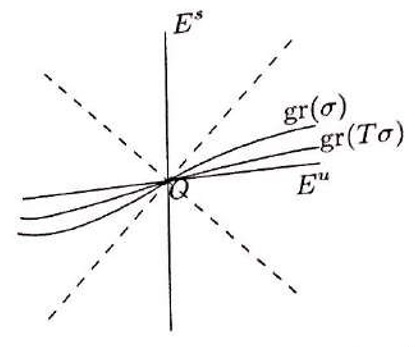
\includegraphics[width=0.6\columnwidth]{2_10.jpg}
\caption{$A + \varphi$ трансформирует граф $\mathrm{gr}(\sigma)$ в граф $\mathrm{gr}(T\sigma)$ порождая отображение, которое трансформирует $\sigma$ в $T\sigma$. Мы должны найти инвариантный граф относительно $A+\varphi$, который соответствует фиксированной точке из $T$ }
\label{fig2_10}
\end{center}
\end{minipage}
\end{center}
\end{figure}



\end{demo}
 


